%-----------------------------------------------------------------------------%
\chapter{\babEmpat}\label{casestudy}
%-----------------------------------------------------------------------------%
There are two case studies used in this research, Charity Organization System and Odoo Sales module. This chapter discuss about those case studies.

%-----------------------------------------------------------------------------%
\section{Charity Organization System (COS)}
%-----------------------------------------------------------------------------%
Charity Organization System (COS)\footnote{http://rse.cs.ui.ac.id/?open=prices/charity} is a system developed to help charity organizations in addressing several issues, such as equal distribution of aid and monitoring process. The development of the system is a part of a project which conducted by researchers in RSE Lab in Faculty of Computer Science UI. There are several charity organizations which will be used this system. Their business processes could be have commonalities, but each charity organization could has different features needed in the system. To address that issue, COS is developed relies on software product line (SPL) approach and uses ABS language. Using SPL approach, each charity organization can choose features based on their need. Then, ABS is one language which relies on SPL approach. By using SPL and ABS, the process of developing each system for each charity organization could be done more efficient.

\begin{figure}
	\centering
	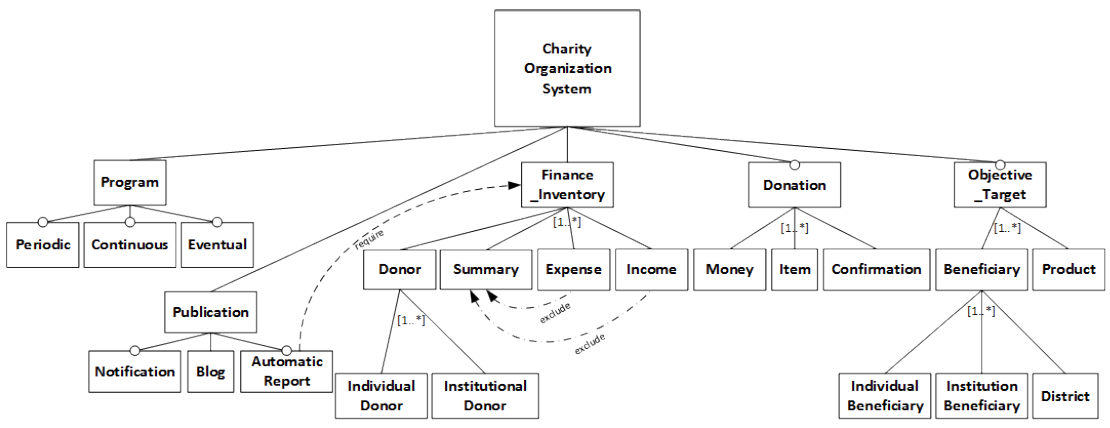
\includegraphics[width=1\textwidth]
	{pics/COSFD.png}
	\caption{Feature Diagram of Charity Organization System}
	\label{fig:COSFD}
\end{figure}

There are several features in COS\footnote{https://gitlab.com/IS4Charity/FeatureDiagram/tree/master/COS}. The feature diagram of COS shown in Figure \ref{fig:COSFD}. Then, the brief explanation of the features is as follow.

\begin{itemize}
	
	\item Program \\
	Types of events carried out by charity organizations.
	\begin{itemize}
		\item Periodic \\
		Event that made within a certain time frame.
		\item Continuous \\
		Event that made routinely.
		\item Eventual \\
		Event that made only one time.
	\end{itemize}
	
	\item Publication \\
	Types of reports used by the charity organizations.
	\begin{itemize}
		\item Notification \\
		An announcement about donations to donors.
		\item Blog \\
		A post about charity activities held.
		\item Automatic Report \\
		An information thath automatically generated from financial data.
	\end{itemize}
	
	\item Finance Inventory \\
	Types of financial records required.
	\begin{itemize}
		\item Donor
		\begin{itemize}
			\item Individual Donor \\
			Record is derived from individual persons.
			\item Institutional Donor \\
			Record is derived from institutions or organizations.
		\end{itemize}
		\item Summary \\
		Recapitulation of the financial report on charities.
		\item Expense \\
		Details of the financial report on expenditures charities.
		\item Income \\
		Details of the financial report on incomes charities.
	\end{itemize}
	
	\item Donation \\
	Types of contributions given in charity events.
	\begin{itemize}
		\item Money \\
		A cash form donation.
		\item Item \\
		A goods form donation.
		\item Confirmation \\
		An acceptance report of delivery donations that have been made.
	\end{itemize}
	
	\item Objective Target \\
	Types of programs aimed to individuals, institutions, or specific places.
	\begin{itemize}
		\item Beneficiary
		\begin{itemize}
			\item Individual Beneficiary
			Individual persons are the target of recipients.
			\item Institution Beneficiary \\
			Institutions or organizations are the target of recipients.
			\item District \\
			Specific area is the target of recipient.
		\end{itemize}
		\item Product
		Program that distributes goods.
	\end{itemize}
\end{itemize}


%-----------------------------------------------------------------------------%
\section{Odoo Sales Module}
%-----------------------------------------------------------------------------%
Odoo is an open-source \citep{web.Odoo.whatIsOdoo,web.Odoo.ERPComparison} enterprise management software \citep{web.Odoo.whatIsOdoo}. It is a suite consists several application modules, such as sales, accounting, manufacturing, purchasing, warehouse management, project management, etc. Odoo is targeting all sizes of companies (small, medium, and large companies). The goals of Odoo are to help the companies to manage, automate, measure and optimize their operations, finances and projects.

As said above, there are several modules in Odoo. One of it is Sales module\footnote{https://www.odoo.com/page/sales}. In Sales module, there are several features which help the users to do sales activity, such as creating quotation, taking sales order, and managing price-lists. Odoo Sales module has 28 features \citep{web.Odoo.OdooSalesFeatures}. The features are as follow.
\begin{itemize}
	\item Quotation Builder. \\
	Build quotation from the predefined products, price lists and templates.
	
	\item Quotation template \\
	Used to design quotation templates that can be reused.
	
	\item Upselling \\
	Quotations are optimized to help users sell more: propose extra options, apply closing triggers, discounts, etc.
	
	\item Electronic Signature \\
	Allow the customers to review and sign their quotations online.
	
	\item Contracts \\
	Record contracts and track invoicing phases, renewal and upselling.
	
	\item Sales Orders \\
	Convert quotation into sales order. Possibility to modify the sales order, remain opened, invoice kits. 
	
	\item Product Variants \\
	Create configurable products with multiple variants (size, color, etc.) and options.
	
	\item Product Types \\
	Manage services, physical products to delivery, electronic products and consumables.
	
	\item Manage invoicing from sales order \\
	Invoicing policy is configured in the product but managed from the sales order.
	
	\item Price-lists \\
	Price-list rules used to compute the right price based on customers conditions. 
	
	\item Dashboard \\
	Get a full overview on personal activities, next actions and performances.
	
	\item Recurring Contracts \\
	Manage subscriptions with Odoo's recurring contracts: billing, renewal alerts, extra options, MRR dashboard, etc.
	
	\item Reduce Data Entry \\
	Send quotes in just a few clicks, manage pipeline with drag and drop, etc.
	
	\item Time and Material Contracts \\
	Invoice customers based on time and materials with contracts.
	
	\item Customer Portal \\
	Customer can get an access to their quotes to track the status sales orders and delivery orders.
	
	\item Milestones \\
	Manage fixed price contract with invoicing based on milestones. Track invoices, forecast revenues and profitability.
	
	\item Discounts \\
	Apply discounts on every lines.
	
	\item Coupons \\
	Create names coupons or shared one to boost customer demands.
	
	\item Order and Invoicing Analysis \\
	Get statistics based on orders and \slash or invoices.
	
	\item Custom Alerts \\
	Follow key quotations and orders and get alerts based on relevant activities.
	
	\item Email Gateways \\
	All email communications automatically attached to the right order.
	
	\item On Boarding Emails \\
	Create template of emails for specific product to give information to buyers: access material, reminder of the service, etc.
	
	\item Multi company rules \\
	Automatically mirror sales orders and purchase orders in multi-company setup.
	
	\item SaaS KPIs \\
	Get a dashboard about all SaaS KPIs: Churn, MRR, Lifetime Value, CAC Ratio, upgrades / downgrades, etc.
	
	\item Modern User Interface \\
	A fast user interface designed for sales. 
	
	\item Mobile \\
	Sell on the road with Odoo's mobile user interface, working even if the users don't have an internet connection.
	
	\item Odoo eSign \\
	Use Odoo eSign to get signatures on NDAs, contracts or any PDF document.
	
	\item Incoterms \\
	Incoterms appear on the invoice.
\end{itemize}

%-----------------------------------------------------------------------------%
\section{Motivation for COS and Odoo Sales Modules Case Study}\label{MotivationCaseStudy}
%-----------------------------------------------------------------------------%
There are several reasons why Charity Organization System and Odoo Sales module chosen to be case study of this research. Those are as follow.

\begin{enumerate}
	\item Charity Organization System 
	\begin{enumerate}
		\item The case study is expected to give an overview concerning the problems in grouping features. This case study has features and  a feature model, but there is no grouping mechanism applied on it.
		\item The case study is addressed actual issues faced by the charity organizations. As stated, charity organizations are facing issues (equal distribution of aid and monitoring process). COS is developed as an intended to help those charity organization addressing the issues.
		\item The case study is developed using SPL approach and ABS language. As COS is developed using SPL approach and ABS language, so there is no need to re-create the system.
	\end{enumerate}
	\item Odoo Sales module
	\begin{enumerate}
		\item The case study is expected to give an overview concerning the problems in grouping features. This case study has features that have no grouping mechanism applied on it.
		\item The case study is expected to represent the scalability of enterprise management software features. An enterprise management software has many features in it. This case study is chosen to represent as a part of the enterprise management software.
		\item The case study is a well-known software with over 2 million users in over 120 countries \citep{web.Odoo.ERPComparison}.
	\end{enumerate}
\end{enumerate}